%---------------------------------------------------------------------
%
%                      resumenManual.tex
%
%---------------------------------------------------------------------
%
% resumenManual.tex
% Copyright 2009 Marco Antonio Gomez-Martin, Pedro Pablo Gomez-Martin
%
% This file belongs to the TeXiS manual, a LaTeX template for writting
% Thesis and other documents. The complete last TeXiS package can
% be obtained from http://gaia.fdi.ucm.es/projects/texis/
%
% Although the TeXiS template itself is distributed under the 
% conditions of the LaTeX Project Public License
% (http://www.latex-project.org/lppl.txt), the manual content
% uses the CC-BY-SA license that stays that you are free:
%
%    - to share & to copy, distribute and transmit the work
%    - to remix and to adapt the work
%
% under the following conditions:
%
%    - Attribution: you must attribute the work in the manner
%      specified by the author or licensor (but not in any way that
%      suggests that they endorse you or your use of the work).
%    - Share Alike: if you alter, transform, or build upon this
%      work, you may distribute the resulting work only under the
%      same, similar or a compatible license.
%
% The complete license is available in
% http://creativecommons.org/licenses/by-sa/3.0/legalcode
%
%---------------------------------------------------------------------
%
% Contiene el cap�tulo del resumen.
%
% Se crea como un cap�tulo sin numeraci�n.
%
%---------------------------------------------------------------------


\chapter{Resumen}
\cabeceraEspecial{Resumen}

\begin{FraseCelebre}
\begin{Frase}
\textexclamdown No est\'ais preparados!
\end{Frase}
\begin{Fuente}
 Illidan Tempestira, World of Warcraft
\end{Fuente}
\end{FraseCelebre}

Los videojuegos pueden ser disfrutados con una amplia variedad de dispositivos de entrada. Desde un mando tradicional hasta unas gafas de realidad virtual pasando por estaciones de simulaci\'on de conducci\'on de coches. Los dispositivos m\'oviles no se quedan atr\'as en ofrecer nuevas posibilidades para jugar a videojuegos. La presencia de estos dispositivos en gran parte de los hogares hace que estos se conviertan en una alternativa a los dispositivos de entrada habituales. Por ello, este proyecto tiene como objetivo la utilizaci\'on de un dispositivo m\'ovil como dispositivo de entrada de juegos ejecutados en el pc. Para ello se ha desarrollado una librer\'ia para el motor de videojuegos Unity y una aplicaci\'on para Android. \\

La herramienta desarrollada se ha probado en un juego para comprobar la usabilidad de la herramienta y su proceso de inclusi\'on. Con este juego se han realizado pruebas de rendimiento para comprobar la velocidad del proceso y ver si la librer\'ia cumpl\'ia los est\'andares de tasas de fotogramas por segundo. Los resultados muestran que este est\'andar es alcanzado por los dispositivos en los que se ha probado.\\

Se pueden encontrar todos los recursos, as\'i como ejecutables, archivos y c\'odigo del proyecto en:\\
\scriptsize

\textbf{\url{https://github.com/sergiojh/ControlRemotoDeVideojuegosConSmartphones}}

\normalsize

\addvspace{1cm}


\Large{\textbf{Palabras claves}}
\normalsize

\addvspace{1cm}

Dispositivo de entrada, m\'ovil, Android, Unity, videojuego, desarrollo de videojuegos


\chapter{Abstract}

Videogames are now enjoy with a variety of input devices. From a tradicional controller to a virtual reality headset including car driving simulation stations. The mobile devices are not far behind in offering new possibilities for video games. The presence of these devices in most of the homes makes these an alternative to tradicional input devices. Therefore, this project aims to use a mobile device as an input device for games played on the pc. Because of this a library for the videogame engine Unity and an app for Android has been developed.\\

The developed tool has been tested in a game to check the usability of the tool and its inclusion process. Performance tests have been performed to verify the speed of the process and see if the library met the frame rate standards. The results show that this standard is achieved by the devices on which it has been tested.\\

All project's resources, executable files, code, and scripts, can be accessed from:\\

\scriptsize

\textbf{\url{https://github.com/sergiojh/ControlRemotoDeVideojuegosConSmartphones}}

\normalsize

\addvspace{1cm}

\huge{\textbf{Keywords}}
\normalsize

\addvspace{1cm}

Input device, phone, Android, Unity, videogame, videogame development

\newpage

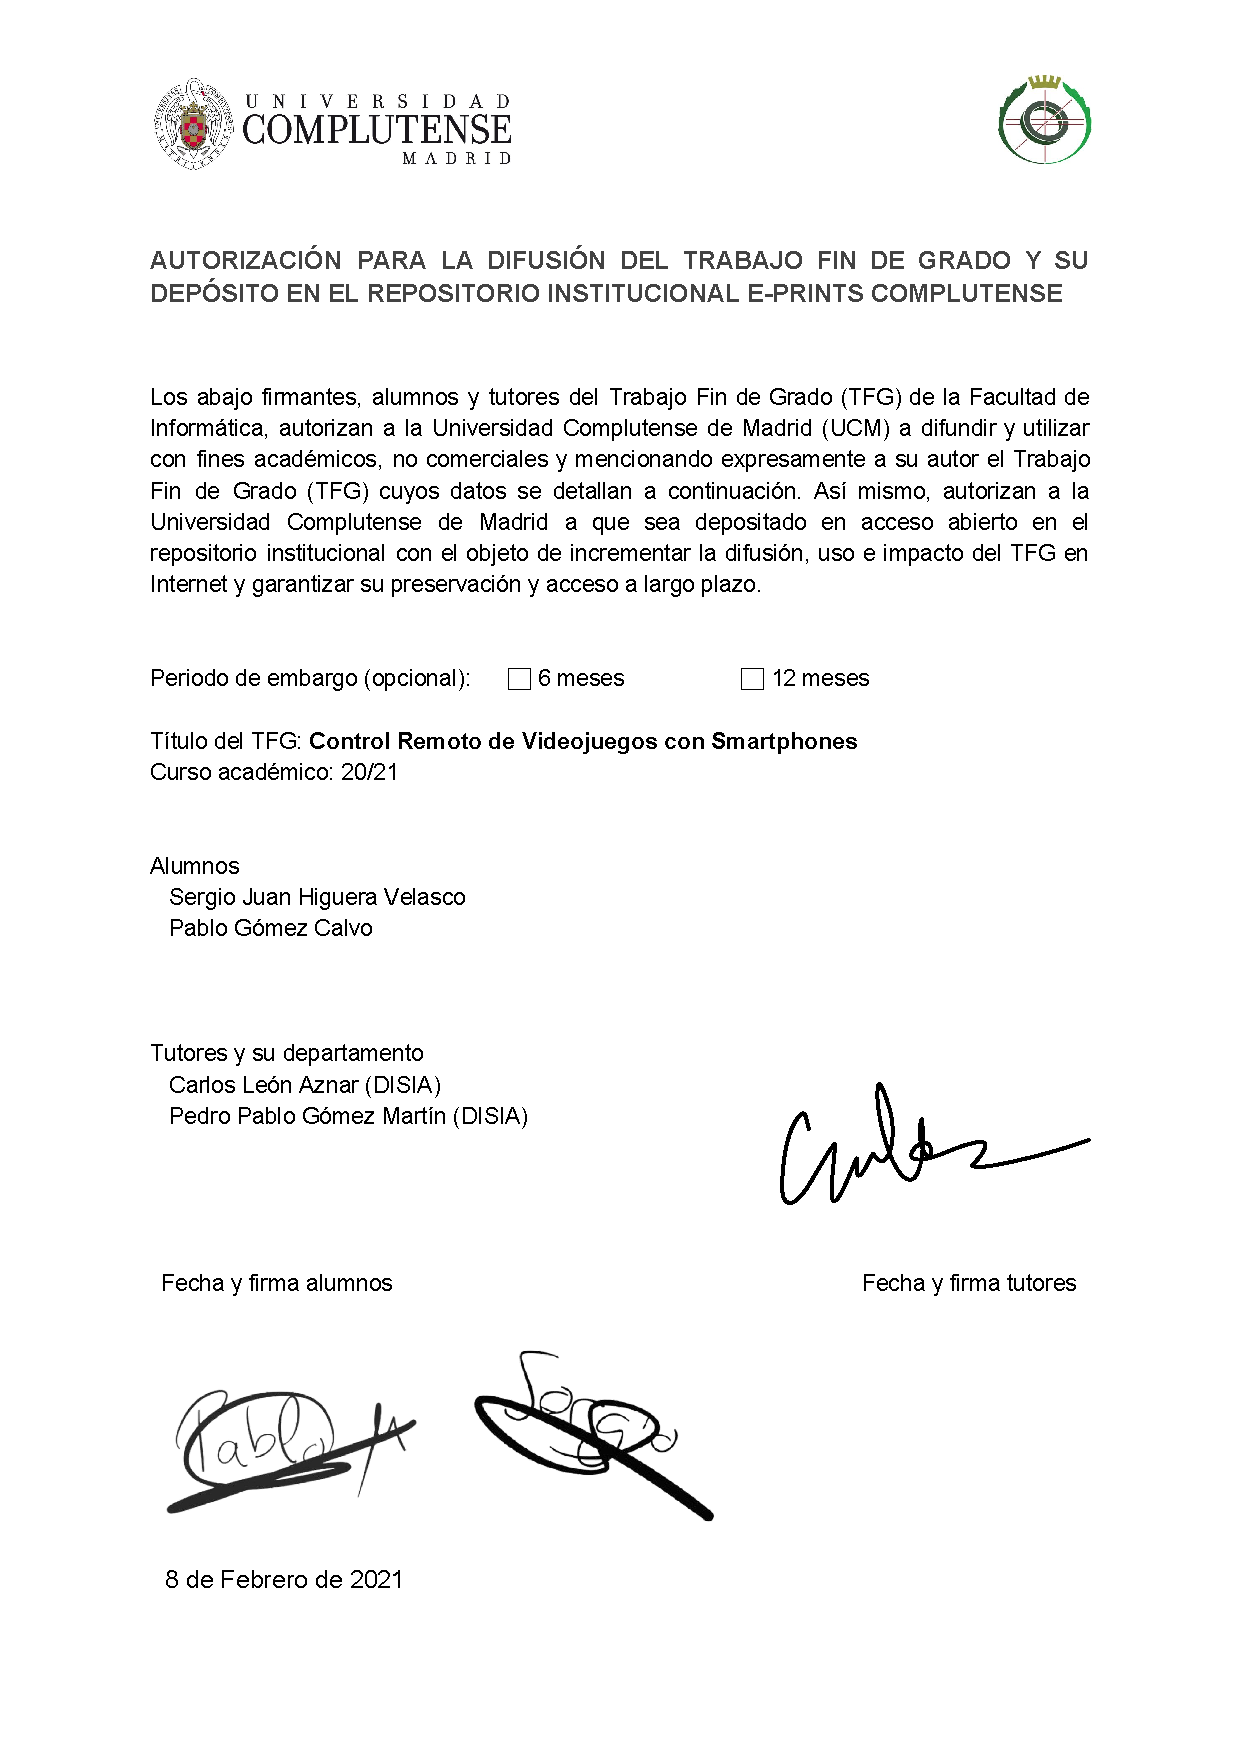
\includegraphics[width=1.0\textwidth]{./Imagenes/Vectorial/Autorizacion.pdf}


\endinput

% Variable local para emacs, para  que encuentre el fichero maestro de
% compilaci�n y funcionen mejor algunas teclas r�pidas de AucTeX
%%%
%%% Local Variables:
%%% mode: latex
%%% TeX-master: "../ManualTeXiS.tex"
%%% End:
